\chapter{User's Manual} \label{sec:manual}

This manual will describe the impedance spectrometer in detail and give step by step instructions for using it.


\section{Overview}

An overview of the device connections can be seen in Figure \ref{fig:device_connections}. Connector footprints for
unimplemented features are not labeled, the push buttons on the board are the same as those on the
STM32F4 Discovery board.

\begin{figure}[htpb]
  \centering
    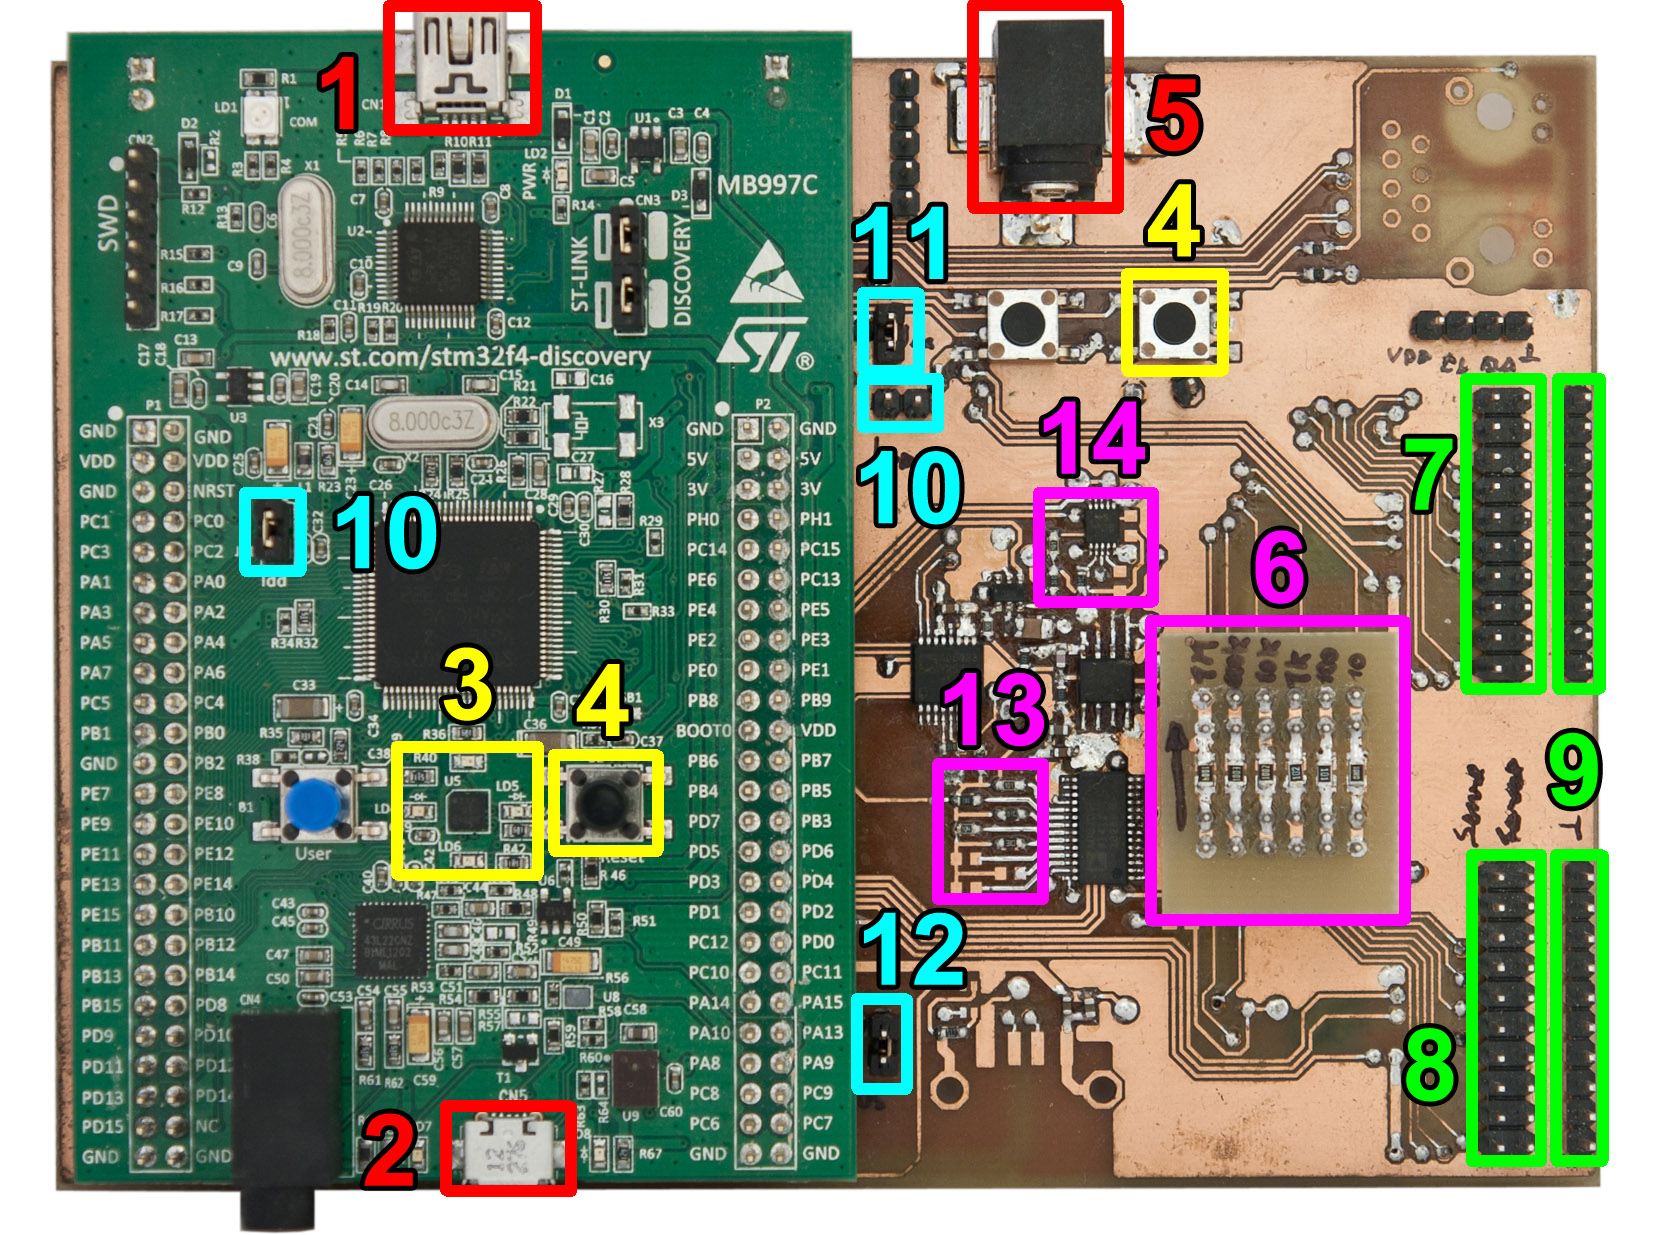
\includegraphics[width=\textwidth]{bilder/device_connections.jpg}
  \caption[Interface on the assembled impedance spectrometer]{
    Interface on the assembled impedance spectrometer:
    \begin{enumerate*}[label=\textbf{\arabic*}, itemjoin={{ -- }}]
      \item USB programming and power connector   \label{itm:usb_prog}
      \item device USB connector   \label{itm:usb_dev}
      \item status LEDs   \label{itm:leds}
      \item reset button   \label{itm:button_rst}
      \item DC power jack   \label{itm:dc_jack}
      \item board with calibration resistors   \label{itm:cal}
      \item measurement output connections, sense (left) and force (right)   \label{itm:meas_out}
      \item measurement input connections (same as output)   \label{itm:meas_in}
      \item ground connections   \label{itm:meas_gnd}
      \item $ I_\text{DD} $ measurement jumper   \label{itm:jump_idd}
      \item $ I_\text{CC} $ measurement jumper   \label{itm:jump_icc}
      \item $ V_\text{BUS} $ jumper   \label{itm:jump_vbus}
    \end{enumerate*} }
  \label{fig:device_connections}
\end{figure}

The USB programming connector \ref{itm:usb_prog} is used to program and debug the device, it can also be used to power
the device from a standard phone charger or similar supply with a Mini-B USB plug.
The device USB connector \ref{itm:usb_dev} is used to connect the device to a PC and control it.
The DC jack \ref{itm:dc_jack} is a standard \unit{2.5}{\milli\meter} jack (center positive) and can be used to
power the device with a \unit{5}{\volt} DC supply.

When using the device with an external power supply, or powered from the programming connector \ref{itm:usb_prog},
the $ V_\text{BUS} $ jumper \ref{itm:jump_vbus} may be disconnected to prevent the board from drawing power from the
device connector \ref{itm:usb_dev}.

The jumpers \ref{itm:jump_idd} and \ref{itm:jump_icc} can be used to measure the current consumption of the
microcontroller and all the other parts, respectively (note that there are two jumpers for $ I_\text{DD} $,
one on the STM32F4 Discovery board and one on the board, and care should be taken to use only one).

There are four status LEDs \ref{itm:leds}, three of which are used at this time:
\begin{itemize}
	\item the \emph{blue} one will blink when the device is powered on, indicating that the firmware hasn't locked up,
  \item the \emph{green} one will light up while a measurement is in progress, allowing the user to see when it has
    finished,
  \item the \emph{red} one will be turned on in case of an error in the firmware, this means the device should be reset
    using the reset button \ref{itm:button_rst} and the steps leading up to the error should be documented to allow
    the programmer to fix it.
\end{itemize}
